%!TEX root = /Users/stevenmartell/Documents/iSCAM-project/fba/Halibut/WRITEUP/Halibut.tex

\section{Model Description} % (fold)
\label{sec:model_description}

The following detailed documentation is a description of the simulation model used to generate model output in this report.  The description is broken down into three subsections: 1) simulation model input, 2) state dynamics, and 3) model outputs.  A series of tables along with a detailed written description is used to document the model.  The tables of equations are meant to represent the logical progression of using input data to initialize the population model, simulating dynamical responses to alternative policies and deriving model outputs.

To summarize the following subsections that describe the model in detail, the following pseudocode represents the general order of operations (implemented as specific functions within the computer code).

\noindent\underline{Pseudocode:}
\begin{enumerate}
	\item Read simulation model inputs, (biological data, fishery data and model parameters).
	\item Initialize model parameters (initial age-structure, annual recruitment, etc).
	\item Calculate length-based selectivities for each gear type for each sex.
	\item Partition fishing mortality to each fishing sector.
	\item Calculate age-specific total mortality rate for each year where the probability of capture and discard is a function of selectivity and size limits.
	\item Calculate numbers-at-age each year based on annual values of $Z$.
	\item Compute model outputs and performance measures.
\end{enumerate}

The underlying model design is and age-structured population model with an annual time step.  The population model has two periods: (1) a historical period in which the population model is initialized with numbers-at-age in the first year, and annual recruitments for each year up to the present, and (2) a projection period where the numbers-at-age are simulated 15 years into the future under alternative scenarios and harvest policy options.  Information for the initialization of the population model is based on the most recent stock assessment for Pacific Halibut \citep{Hare2012Rara}.  At each time step in the model, total age/sex-specific mortality rates are computed as a sum of natural and fishing mortalities from each of the directed and non-directed fisheries.

The detailed analytical description of the simulation model that follows is arranged in a series of tables of equations that are intended to provide a concise description, as well as, provide the logical order of operations in which the code is executed.  A list of parameter symbols, the units, and description is provided in Table \ref{tab:ListOfSymbols}.  The source code for this simulation model can also be obtained from a code.google repository at \url{http://code.google.com/p/iscam-project/}.


%%NOTES TO BE INCLUDED 
Permitted bycatch mortality in BSAI groundfish fisheries in 2012 are 900 mt for the fixed gear and 3,525 mt for the trawl gear.  The accounting system for trawl by catch is that 80\% of the net halibut weight landed is assumed to die, and in the case of the pollock fishery a 90\% discard mortality is assumed.

% -----------------------------------------------------------------------------
\subsection{Simulation model input} % (fold)
\label{sub:simulation_model_input}

Input data for the simulation model was provided by Steve Hare from the IPHC in the form of the report file from the assessment model presented at the 2012 annual meeting \citep{Hare2012Rara}.  The input data for the simulation model, along with the control file and initial parameter value can be found in appendix \ref{appen:dataFiles}.  The following list is a summary description of the model inputs that are required to run the simulation model.

List of model input:
\begin{enumerate}
	\item Model dimensions (i.e., years, number of gears, number of age-classes).
	\item Historical catch data and fishing mortality rates for 5 gear types.
	\item Annual recruitment from 1996 to present.
	\item Initial numbers-at-age (2-30) by sex.
	\item Selectivity parameters (length-based selectivity).
	\item Size limit, target harvest rate, \& other policy related parameters (e.g., SUFD).
\end{enumerate}

The model dimensions are consistent with the IPHC assessment model where the model starts in 1996 and is conditioned on the assessment data through 2011, the number of ages ranges from 1--30, and the fisheries are broken down into five distinct components: 
\begin{enumerate}
	\item the setline fishery (including the IPHC research catch),
	\item the sublegal discards (including U32 wastage and U32 bycatch),
	\item the fully recruited by catch (O32 wastage and bycatch),
	\item the recreational sport fishery, and
	\item and the personal use (subsistence fishery).
\end{enumerate}
Each of these `gears' have there own length-based selectivity coefficients and fishing mortality rates that are based on the most recent assessment model output.  The historical catch data for each of these gears are also given in the input data, but are not used to calculate total mortality rates in anyway.  




\begin{table}[ht]
	\caption{List of symbols, units and description of variables for the simulation model.}
	\label{tab:ListOfSymbols}
	\begin{center}
	\begin{tabular}{ccl}
		\hline
		Symbol & Units & Description \\
		\hline
		$h$	& - & index for sex\\
		$i$	& - & index for year\\
		$j$	& - & index for age\\
		$k$	& - & index for gear\\
		$l$ & - & index for length\\
		\multicolumn{3}{l}{\underline{Input Parameters}}\\
		$R_0$	& millions	& unfished recruitment\\
		$h$		& -			& steepness of the stock-recruitment relationship\\
		$M_h$	& yr$^{-1}$	& instantaneous natural mortality rate by sex (0.15 female, 0.135 male). \\
		$\bar{R}$ & millions & average recruitment\\
		$\ddot{R}$ & millions & initial recruitment\\
		$\omega_i$ & - & annual recruitment deviation in year $i$ (assume 50:50 sex ratio at age-1)\\
		$\ddot{\omega}_{h,j}$ & - & initial recruitment deviation for sex $h$ and age $j$\\
		\multicolumn{3}{l}{\underline{Dynamic Variables}}\\
		$F_{h,i,k}$ & yr$^{-1}$ & Fishing mortality rate by sex $h$ in year $i$, for gear $k$\\
		$s_{h,l,k}$ & - & log selectivity for sex $h$, length $l$ for gear $k$\\
		$\nu_{h,i,j,k}$ & - & log selectivity for sex $h$, year $i$, age $j$ in gear $k$\\
		$Z_{h,i,j}$ & yr$^{-1}$ & Age-specific total mortality rate for sex $h$ in year $i$\\
		$N_{h,i,j}$ & millions & numbers of halibut of sex $h$, in year $i$, at age $j$\\
		$SB_{i}$ & million pounds & Female spawning biomass in year $i$\\
		\hline
	\end{tabular}
	\end{center}
\end{table}

% subsection simulation_model_input (end)
% -----------------------------------------------------------------------------
\subsection{Analytical description} % (fold)
\label{sub:analytical_description}

% 1) Initial states
\subsubsection{Initial states ($i$=1996:2011)} % (fold)
\label{ssub:initial_states}
The simulation model is initialized using the model estimates of numbers-at-age and annual recruitment produced by the IPHC 2011 halibut stock assessment \citep{Hare2012Rara}.  Two parameter vectors, $\Theta$ and $\Phi$ are used to categorize population parameters as sex independent and dependent, respectively.  Components of these two vectors are defined in \eqref{T1.1} and \eqref{T1.2}, where $R_0$ and $h$ define the unfished age-1 recruits and steepness of the stock recruitment relationship.  Note that these terms ($R_0,h$) are not of interest in this simulation model, because we do not use a stock recruitment relationship to simulate future recruitment.  The average recruitment $\bar{R}$ and annual deviations $\omega_i$ are used to initialize age-1 recruits from 1996 to 2011 \eqref{T1.7}, where these values were obtained from the IPHC assessment report file.  The sex-specific parameters $\Phi$ consists of the initial average recruitment $\ddot{R}_{h}$ and cohort specific deviations $\ddot{\omega}_{j}$ which makes up the initial numbers at age in 1996 \eqref{T1.7}.  Sex-specific natural mortality $M_h$ rates were set at 0.15 and 0.135 for females and males, respectively.  The annual fishing mortality rates $f_{h,i,k}$ (on a log scale) for sex, year, and gear were taken from the IPHC assessment along with the selectivity coefficients $s_{h,l,k}$ (also on a log scale) for sex, length, and gear.  Age-specific selectivities for each gear, year, and sex ($\nu_{h,i,j}$) were based on a piece-wise liner interpolation \eqref{T1.4} of the length-based selectivity coefficients $S_{h,i,k}$ and the mean length-at-age $l_{h,i,j}$ in the annual IPHC setline survey \eqref{T1.3}.  In \eqref{T1.4} the $l^{(0)}$ and $l^{(1)}$ terms correspond to the length intervals on either side of the current $l_{h,i,j}$ values (Note that this function is equivalent to the \texttt{approx} function implemented in the R-scripting  \citep{R-Development-Core-Team:2009fk} language).  Annual sex- age-specific fishing mortality rates are based on \eqref{T1.5} for each gear $k$, and the total mortality is the sum of natural and fishing mortalities \eqref{T1.6}.

\begin{table}
	\caption{Analytical description of the sex-based age-structured model used for simulation projections.}
	\label{tab:model_description}
	\begin{center}
		\tableEq
		\begin{align}
			\hline \nonumber\\
			&\mbox{Model parameters} \nonumber\\
			\Theta &= \{R_0,h,\bar{R},\omega_{i}\}  \label{T1.1}\\
			\Phi   &= \{\ddot{R}_h,\ddot{\omega}_{h,j},M_h,f_{h,i,k},s_{h,l,k},a_{50},\gamma_{50}\}  \label{T1.2}\\
			%
			&\mbox{Input data} \nonumber\\
			&C_{i,k}, l_{h,i,j},w_{h,i,j} \label{T1.3}\\
			%
			&\mbox{Initialize state variables }\nonumber\\
			\nu_{h,i,j} &= s_{h,l}^{(0)}+ 
			\frac{ (l_{h,i,j}-l^{(0)})s_{h,l}^{(1)} - (l_{h,i,j}-l^{(0)})s_{h,l}^{(0)} }
			{ l^{(1)}-l^{(0)} }, \quad \mbox{where}
			\quad  l^{(0)} \leq l_{h,i,j} \leq l^{(1)} \label{T1.4}\\
			F_{h,i,j,k} &= \exp(f_{h,i,k} + \nu_{h,i,j,k}) \label{T1.5}\\
			Z_{h,i,j} & = M_h + \sum_k F_{h,i,j,k} \label{T1.6} \\
			&\mbox{Numbers at age}\nonumber\\
			N_{h,i,j} &= 
			\begin{cases}
				\ddot{R}_{h}\exp(\ddot{\omega}_{h,j}-M_h (j-1)), & \mbox{for $2<j<30$}\\
				0.5 R_h\exp(\omega_{i}), \quad \mbox{for $1996<i<2026$}\\
			\end{cases} \label{T1.7}\\
			%
			N_{h,i+1,j+1} &= N_{h,i,j} \exp(-Z_{h,i,j}), \quad \mbox{for 1$<j<$ 30}\label{T1.8}\\
			N_{h,i+1,j} &= N_{h,i,j-1}+N_{h,i,j} \exp(-Z_{h,i,j}) , 
			\quad \mbox{for $j =$30}\label{T1.9}\\
			%
			&\mbox{Model outputs}\nonumber\\
			%
			SB_{i} &= \sum_{j=6}^{j=30} N_{h,i,j}\exp(-0.5Z_{h,i,j}) p_{h,j} w_{h,i,j},
			\quad \mbox{where $h=1$}\label{T1.10}\\
			%
			C_{i,k} &=\sum_h \sum_j \frac{N_{h,i,j} w_{h,i,j} f_{h,i,k} s_{h,i,j}
			(1-\exp(-Z_{h,i,j}))}{Z_{h,i,j}}\label{T1.11}\\
			%
			EB_{i} &= \sum_h \sum_{j=6}^{j=30} N_{h,i,j} w_{h,i,j} \exp(\nu_{h,i,j,k=1}) \label{T1.12}\\
			%
			YBio_i &= \sum_h \sum_j \frac{N_{h,i,j}w_{h,i,j}f_{h,i,k=1}s_{h,i,j,k=1} r_{h,i,j,k=1}(1-\exp(-Z_{h,i,j}))}
			{Z_{h,i,j}}\label{T1.13}\\
			%
			WBio_i &= \sum_h \sum_j
			\frac{N_{h,i,j}w_{h,i,j}f_{h,i,k=1}s_{h,i,j,k=1}(1-r_{h,i,j,k=1})d_{k=1}(1-\exp(-Z_{h,i,j}))}
			{Z_{h,i,j}} \label{T1.14}\\
			%
			LBio_i &= YBio_i^{(f_{k=2,3}=0)} - YBio_i \label{T1.15}\\
			%
			BBio_i &= \sum_h \sum_j \sum_{k=2}^{k=3}
			\frac{N_{h,i,j}w_{h,i,j}f_{h,i,k}s_{h,i,j,k} r_{h,i,j,k}(1-\exp(-Z_{h,i,j}))}
			{Z_{h,i,j}}\label{T1.16}\\
			%
			YLR_i & = \frac{LBio_i}{BBio_i}\label{T1.17}\\
			\hline \nonumber
		\end{align}
		\normalEq
	\end{center}
\end{table}

The numbers-at-age by sex are initialized using \eqref{T1.7} and are updated using \eqref{T1.8} and \eqref{T1.9} for the plus group.  Female spawning biomass each year is calculated as the product of the number of females surviving half the $Z$ in a given year, the proportion mature-at-age, and the observed average catch weight-at-age $w_{h,i,j}$ in a given year.  Prior to 2001, aging data ranged from age-6 to age-20, and post 2001 break and burn methods were used to age halibut upto age-25, where 25 is the new plus group.  This calculation \eqref{T1.10} of spawning biomass differs slightly from the IPHC code, where the numbers-at-age each year are smeared by an aging error matrix, and the average weight at age from the survey was used. The predicted catch in year $i$ for gear $k$ is given by \eqref{T1.11}, which is the sum over the catch-at-age by sex.

% subsubsection initial_states (end)
% 2) Selectivities and joint probablity for fishing mortality & discard mortality.
\subsubsection{Joint probability model for fishing \& discard mortality} % (fold)
\label{ssub:joint_probability_for_fishing_&_discard_mortality}
For the future simulations ($i\geq$ 2012), the directed setline fishery for halibut is based on the probability of capturing a fish of age $j$ times the probability of retaining a fish of age $j$.  This joint probability is represented by the age-selectivity of the fishing gear (which is a length-based function) and variation in growth of male and female halibut.  The age-based selectivity is based on \eqref{T1.4}.  The probability of retaining a fish of age $j$ is the based on the probability of an age $j$ fish being larger than the size limit. This integral was approximated using a logistic function of the mean length-at-age and assuming a coefficient of variation of 0.1 in length-at-age such that the standard deviation in length-at-age $\sigma_j$ increases as a linear function of length:
\[
p(r)_j = \frac{1}{1+\exp(-(l_j-\mathrm{MSL})/\sigma_j)}
 \] 
The probability of discarding a fish of age $j$ is defined as $1-p(r)_j$.  Figure \ref{fig:FIGURES_SIZELIMIT_SelRetA} shows how retention and discarding probabilities vary with age with a 32 inch size limit in place.  Note that when the mean length-at-age gets smaller, this retention probability shifts to the right (older ages) and fish recruit to the fishing gear later in life.
\begin{figure}[htbp]
	\centering
		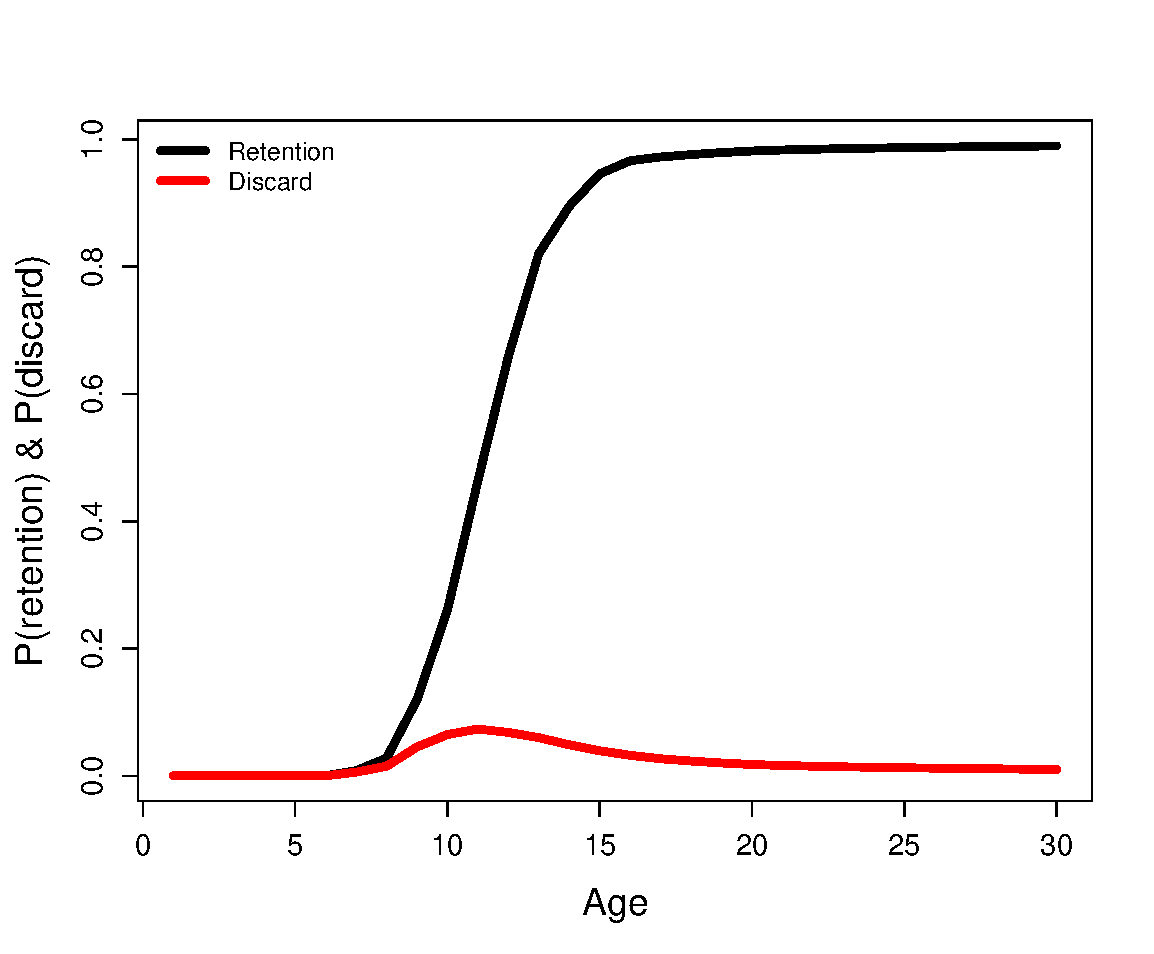
\includegraphics[height=3in]{../FIGURES/SIZELIMIT/SelRetA.pdf}
	\caption{Probability of retention and discarding a  halibut with a 32 inch size limit in place.}
	\label{fig:FIGURES_SIZELIMIT_SelRetA}
\end{figure}

% subsubsection joint_probability_for_fishing_&_discard_mortality (end)

% 3) Calculating fishing mortality rates from 1994-present conditioned on catch.
In the more recent stock assessment models, the age/sex/size composition of the commercial landings are estimated externally to the model.  These data were not available to be used in this analysis. For the 1996 to 2011 period, fishing mortality rates were taken from the IPHC assessment model.  For the projection period ($i>2011$), fishing mortality rates were based on the projected catches for each of the five gears (commercial, U32, O32, recreational, personal). Sex-specific fishing mortality rates were determined using a numerical procedure to solve the Baranov catch equation \eqref{T1.11}.  An initial guess for the sex-specific fishing rate $f_{h,i,k}$ for gear $k$ in year $i$, followed by the use of Newtons' root finding method to find the appropriate values of $f_{h,i,k}$ such that the sum of the predicted female and male catches for each gear was equivalent to the catch allocated to that gear.  
% subsection analytical_description (end)
% -----------------------------------------------------------------------------
\subsection{Model outputs} % (fold)
\label{sub:model_outputs}
Simulation model outputs of interest for this study are:
\begin{enumerate}
	\item Exploitable biomass,  EBio defined by \eqref{T1.12}.
	\item Female spawning biomass, SBio defined by \eqref{T1.10}.
	\item Commercial Yield, YBio defined by \eqref{T1.13}.
	\item Wastage from the commercial fishery, WBio defined by \eqref{T1.14}.
	\item Lost yield due to bycatch from non-directed fisheries, LBio defined by \eqref{T1.15}.
	\item Bycatch from non-directed fisheries, BBio defined by \eqref{T1.16}.
	\item The yield loss ratio, YLR defined by \eqref{T1.17}.
\end{enumerate}

Note that in order to calculate the lost yield \eqref{T1.15}, the model was run as if there were no bycatch of halibut in other fisheries, and all of the available CEY for each area was allocated to the commercial gear.  The lost yield is the difference between the yield obtained with no bycatch and the yield obtained with bycatch allotments in place.


% subsection model_outputs (end)


% section model_description (end)

